\documentclass[]{article}
\usepackage{lmodern}
\usepackage{amssymb,amsmath}
\usepackage{ifxetex,ifluatex}
\usepackage{fixltx2e} % provides \textsubscript
\ifnum 0\ifxetex 1\fi\ifluatex 1\fi=0 % if pdftex
  \usepackage[T1]{fontenc}
  \usepackage[utf8]{inputenc}
\else % if luatex or xelatex
  \ifxetex
    \usepackage{mathspec}
  \else
    \usepackage{fontspec}
  \fi
  \defaultfontfeatures{Ligatures=TeX,Scale=MatchLowercase}
\fi
% use upquote if available, for straight quotes in verbatim environments
\IfFileExists{upquote.sty}{\usepackage{upquote}}{}
% use microtype if available
\IfFileExists{microtype.sty}{%
\usepackage{microtype}
\UseMicrotypeSet[protrusion]{basicmath} % disable protrusion for tt fonts
}{}
\usepackage[margin=1in]{geometry}
\usepackage{hyperref}
\hypersetup{unicode=true,
            pdftitle={Individual participant data meta-analysis. When? Why? How? A scoping review},
            pdfauthor={Michail Belias},
            pdfborder={0 0 0},
            breaklinks=true}
\urlstyle{same}  % don't use monospace font for urls
\usepackage{graphicx,grffile}
\makeatletter
\def\maxwidth{\ifdim\Gin@nat@width>\linewidth\linewidth\else\Gin@nat@width\fi}
\def\maxheight{\ifdim\Gin@nat@height>\textheight\textheight\else\Gin@nat@height\fi}
\makeatother
% Scale images if necessary, so that they will not overflow the page
% margins by default, and it is still possible to overwrite the defaults
% using explicit options in \includegraphics[width, height, ...]{}
\setkeys{Gin}{width=\maxwidth,height=\maxheight,keepaspectratio}
\IfFileExists{parskip.sty}{%
\usepackage{parskip}
}{% else
\setlength{\parindent}{0pt}
\setlength{\parskip}{6pt plus 2pt minus 1pt}
}
\setlength{\emergencystretch}{3em}  % prevent overfull lines
\providecommand{\tightlist}{%
  \setlength{\itemsep}{0pt}\setlength{\parskip}{0pt}}
\setcounter{secnumdepth}{0}
% Redefines (sub)paragraphs to behave more like sections
\ifx\paragraph\undefined\else
\let\oldparagraph\paragraph
\renewcommand{\paragraph}[1]{\oldparagraph{#1}\mbox{}}
\fi
\ifx\subparagraph\undefined\else
\let\oldsubparagraph\subparagraph
\renewcommand{\subparagraph}[1]{\oldsubparagraph{#1}\mbox{}}
\fi

%%% Use protect on footnotes to avoid problems with footnotes in titles
\let\rmarkdownfootnote\footnote%
\def\footnote{\protect\rmarkdownfootnote}

%%% Change title format to be more compact
\usepackage{titling}

% Create subtitle command for use in maketitle
\providecommand{\subtitle}[1]{
  \posttitle{
    \begin{center}\large#1\end{center}
    }
}

\setlength{\droptitle}{-2em}

  \title{Individual participant data meta-analysis. When? Why? How? A scoping
review}
    \pretitle{\vspace{\droptitle}\centering\huge}
  \posttitle{\par}
    \author{Michail Belias}
    \preauthor{\centering\large\emph}
  \postauthor{\par}
      \predate{\centering\large\emph}
  \postdate{\par}
    \date{May 13, 2019}

\usepackage{booktabs}
\usepackage{longtable}
\usepackage{array}
\usepackage{multirow}
\usepackage{wrapfig}
\usepackage{float}
\usepackage{colortbl}
\usepackage{pdflscape}
\usepackage{tabu}
\usepackage{threeparttable}
\usepackage{threeparttablex}
\usepackage[normalem]{ulem}
\usepackage{makecell}
\usepackage{xcolor}

\begin{document}
\maketitle

\hypertarget{abstract-200-words}{%
\section{Abstract (200 words)}\label{abstract-200-words}}

\hypertarget{background}{%
\subsection{Background}\label{background}}

Individual participant data(IPD) meta-analysis(MA) is considered the
gold standard for evidence based inference. It is well established that
IPD-MA offers great advantages compared to aggregate MA and single
studies. Nevertheless, it is unclear which advantages are mostly
addressed when IPD-MAs are conducted. Furthermore, it is unclear which
statistical approaches are preferred, how they are the results
presented, which medical fields are involved and to what extent
guidelines are followed. \textbf{Objective:} Our objective is to conduct
a scoping review of existing IPD-MA, and summarise their properties.
Furthermore, we aim to inform when and how IPD-MA are performed, whether
state-of the art methods are used and whether they are clearly
described.

\emph{We can propose the use of a statistical ID}

\hypertarget{methods}{%
\subsection{Methods}\label{methods}}

We performed a scoping review to identify IPD-MA performed the last five
years. We searched MEDLINE and the Cochrane Library for IPD-MA, written
in English and from 01/01/2015 to 01/05/2019 time period. We included
both IPD meta-analyses of randomised clinical trials and observational
studies, but excluded diagnostic IPD-MA. We screened the abstracts and
extracted their goal.

\textbf{(we can include more databases i.e.~EMBASE etc)}

\hypertarget{results}{%
\subsection{Results}\label{results}}

Our search resulted in 1538 articles. We included only IPD-MAs with at
least one treatment comparison. We showed an increase per year in
IPD-MAs performed. The two most predominant medical fields were Cancer
\emph{(16\%)}, Cardiovascular diseases \emph{(16\%)} and Mental health
\emph{(10\%)}. Nevertheless, more information should be provided in both
the abstract and the article over the statistical approaches followed.\\
\textbf{An increasing trend in one-stage methods frequency by year has
been showed. Most of the IPD-MAs had as a goal to investigate for
subgroups effects. Reporting type of }

\hypertarget{conclusions}{%
\subsection{Conclusions}\label{conclusions}}

Goal and statistical approach description is still unclear. One-stage
methods are increasing per year. Subgroups analysis is not the primary
goal of IPD-MAs.

\newpage

\hypertarget{introduction}{%
\section{Introduction}\label{introduction}}

Meta-analysis (MA) is a statistical method that involves combining
information from multiple sources. While initially, meta-analyses were
limited in aggregated data (AD) in the early 1990s individual
participant data meta-analysis (IPD-MA or IPDMA) was introduced
(CHALMERS 1993). In IPD-MA the participant level information is
available and therefore evidence from multiple studies can be analysed
centrally. Collecting the IPD may be a difficult and time consuming
task, but neverthetheless IPD-MA is considered the gold standard in
evidence synthesis (Stewart and Parmar 1993 ; and 1995 ; Stewart and
Tierney 2002) and offers great opportunities (Walraven 2010) that in
AD-MA are considered impossible. Besides when investigating overall
treatment effects where AD-MA and IPD-MA are mathematically equivalent,
IPD-MA offers (1) the possibility to standardize subgroup definitions
and outcomes across studies, (2) higher validity and credibility of
subgroup findings, (3) increased flexibility to search for subgroups
based on combinations of patient and/or disease characteristics (4) the
possibility to avoid ecological BIAS (5) investigate non-linear
functional forms (6) training better prediction models and (7)
efficiently synthesizing evidence from different designs. \emph{we can
place extra stuff}

\textbf{Reporting} IPD-MA may be conducted in either one stage or two
stages. In one-stage IPD-MA, a statistical model of choice is applied
and IPD from all studies are analysed simultaneously, whilst accounting
for within-studies clustering of the participants. On the other hand, in
two-stage IPD-MA a statistical model of choice is fitted per study.
Subsequently the estimates extracted are pooled using inverse-variance
meta-analytical methods. Both approaches have a variety of parameters
and results that should be reported in the abstract, the methods and the
results section. An extented version of PRISMA for IPD (Stewart et al.
2015) offers guidance on how to report results in IPD-MA. For instance,
in two-stage IPD-MA 1) heterogeneity measures ( \(I^2\) , Cochran's Q
\(\tau^2\)) 2) and their corresponding methods used 3) forest plots (if
applicable) and 4) use of fixed or random effects models and any other
model assumptions should be described in the Methods section.
Furthermore, in't Hout (IntHout et al. 2016) suggested that prediction
intervals of estimates are also a valuable information and sould be
included. On the other hand, in one-stage IPD-MA 1) specification of
one-stage models 2) use of fixed-effect, stratified or random-effects in
the terms of the model and 3) how clustering of patients within studies
was accounted for should be reported in the methods section.

\textbf{Effect modification} Simmonds et al.~(Simmonds, Stewart, and
Stewart 2015) showed that IPD-MA are frequently performed in order to
detect treatment effect modificaiton. The approaches that were mostly
used were one agreegated data meta-analysis approach `meta-regression'
and three IPD-MA approaches, per-subgroup meta-analysis, meta-analysis
of interaction terms and one-stage IPD-MA. Guidance on which method to
choose is available. Specifically, Simmnond and Higgins (Simmonds and
Higgins 2007) mathematically proved that, given some unrealistic
assumptions, one-stage IPD-MA is always more powerful than meta-analysis
of interaction terms and meta-regression. Fisher et al.~(Fisher et al.
2011) also critically reviewed all four approaches. They concluded that
one-stage IPD-MA allows for more complex analysis, but is more difficult
to perform than pooling within-trial interaction terms. Furthermore, Hua
et al.~(Hua et al. 2016) noted that these one-stage IPD-MA using
mixed-effects modeling should also centre the effect modifiers to their
mean, in order to separate across and within trial information and
therefore accounting for ecological bias.

\textbf{Modeling functional forms} IPD-MA may be performed in order to
investigate the role of risk-factors in the prevalence of a disease. In
that case observational studies are typically meta-analysed. Thereto,
IPD-MA may involve modeling also non-linear functional forms. Sauerbrei
and Royston (Sauerbrei and Royston 2011) suggested the use of a two
stage approach. As a first stage a fractional polynomial is selected and
pooling their estimates through a point-wise weighted meta-analytical
process. Subsequently they extended these non-linear associations to
include interactions (Royston and Sauerbrei 2013). Furthermore, splines
may also be applied to detect non-linear associations.

\textbf{Reviews like ours and goal} So far systematic reviews over the
IPD-MA practices are limited until 2014. For instance, Simmonds et al
(Simmonds et al. 2005) identified 44 IPD-MAs performed during 2000-2005
time period and 1) summarized whether IPD-MAs obtained all the data they
sought 2) reported the types of approaches that were used in the
analysis 3) and whether the effects of covariates have been investigated
and 4) report which medical field was their topic. On a subsequent
paper, 10 years kater Simmonds et al.~(Simmonds, Stewart, and Stewart
2015) identified 1371 potential IPD-MAs performed during 2010-2015 time
period, sampled 184 of them and after obtaining full texts included 100
IPD-MAs. Then they investigated along with the topics investiagted in
the initial paper they investigated also the quality of IPD-MA
reporting. Riley et al.~(Riley, Lambert, and Abo-Zaid 2010) identified
383 IPD-MAs performed form instance until 2009 and summarised 1) theier
medical field topic and 2) whether they assessed risk or prognostic
factors. Finally, Schuit and Ioannidis (Schuit, Li, and Ioannidis 2018)
identified 327 IPD-MAs performed from inception until 2014.
Nevertheless, they restricted their interest in subgroup effects
investigation. Our objective is to conduct a systematic review of IPD-MA
from 2015 onwrds and and summarise their properties. Furthermore, we aim
to inform when and how IPD-MA are performed, whether state-of the art
methods are used and whether they are clearly described.

\newpage

\hypertarget{methods-1}{%
\section{Methods}\label{methods-1}}

This study is a scoping review of IPDMAs, i.e.~a meta-epidemiological
assessment. We report our study according to the Preferred Reporting
Items for Systematic Reviews and Meta-Analyses (PRISMA) guidelines.

\hypertarget{ipd-ma-search-and-selection-strategy}{%
\subsection{IPD-MA search and selection
strategy}\label{ipd-ma-search-and-selection-strategy}}

We searched MEDLINE, pubmed, Cochrane library \textbf{(we can place
more)} for IPD-MA conducted from 01/01/2015 until 01/05/2019, query in
\emph{Supplementary material}.

\newpage

\hypertarget{results-1}{%
\section{Results}\label{results-1}}

We identified 1538 IPD-MAs. s

\begin{table}[t]

\caption{\label{tab:unnamed-chunk-2}Figure 1}
\centering
\begin{tabular}{lr}
\toprule
Var1 & Freq\\
\midrule
Anaesthesiology & 1\\
Cancer & 20\\
Cardiovascular disease & 34\\
Child health & 18\\
Ear, nose and throat & 1\\
\addlinespace
Endocrine and metabolic & 10\\
Gastroenterology & 8\\
Generic Care & 3\\
Geriatrics & 3\\
Gynaecology & 1\\
\addlinespace
Infectious disease & 3\\
Lungs and airways & 5\\
Mental health & 24\\
Neurology & 30\\
Nutrition & 1\\
\addlinespace
Orthopedics & 6\\
Other & 1\\
Pregnancy and childbirth & 18\\
Psychology & 3\\
Renal Disease & 1\\
\addlinespace
Review & 2\\
Statistical & 11\\
Vaccines & 2\\
Wound & 1\\
\bottomrule
\end{tabular}
\end{table}

\begin{verbatim}
## TypeError: Attempting to change the setter of an unconfigurable property.
## TypeError: Attempting to change the setter of an unconfigurable property.
\end{verbatim}

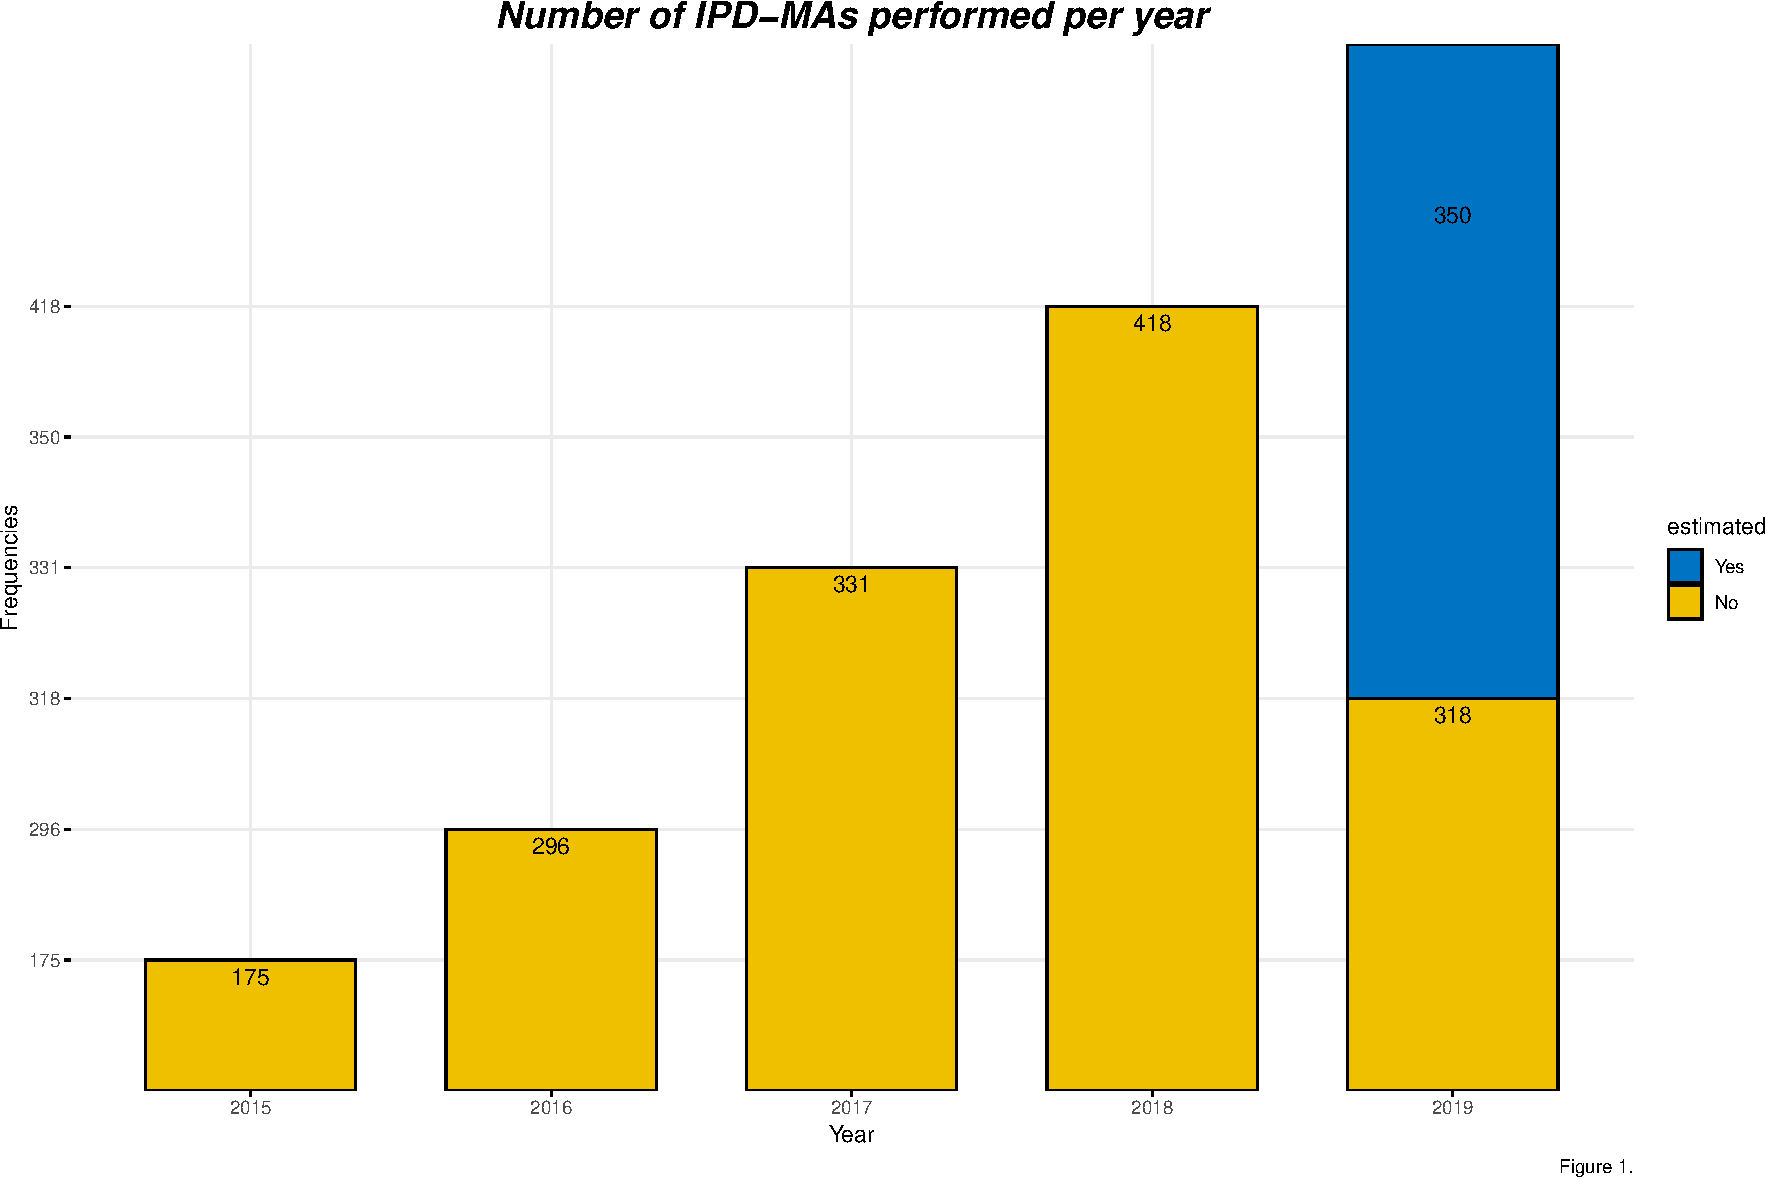
\includegraphics{Figs/unnamed-chunk-3-1.pdf}

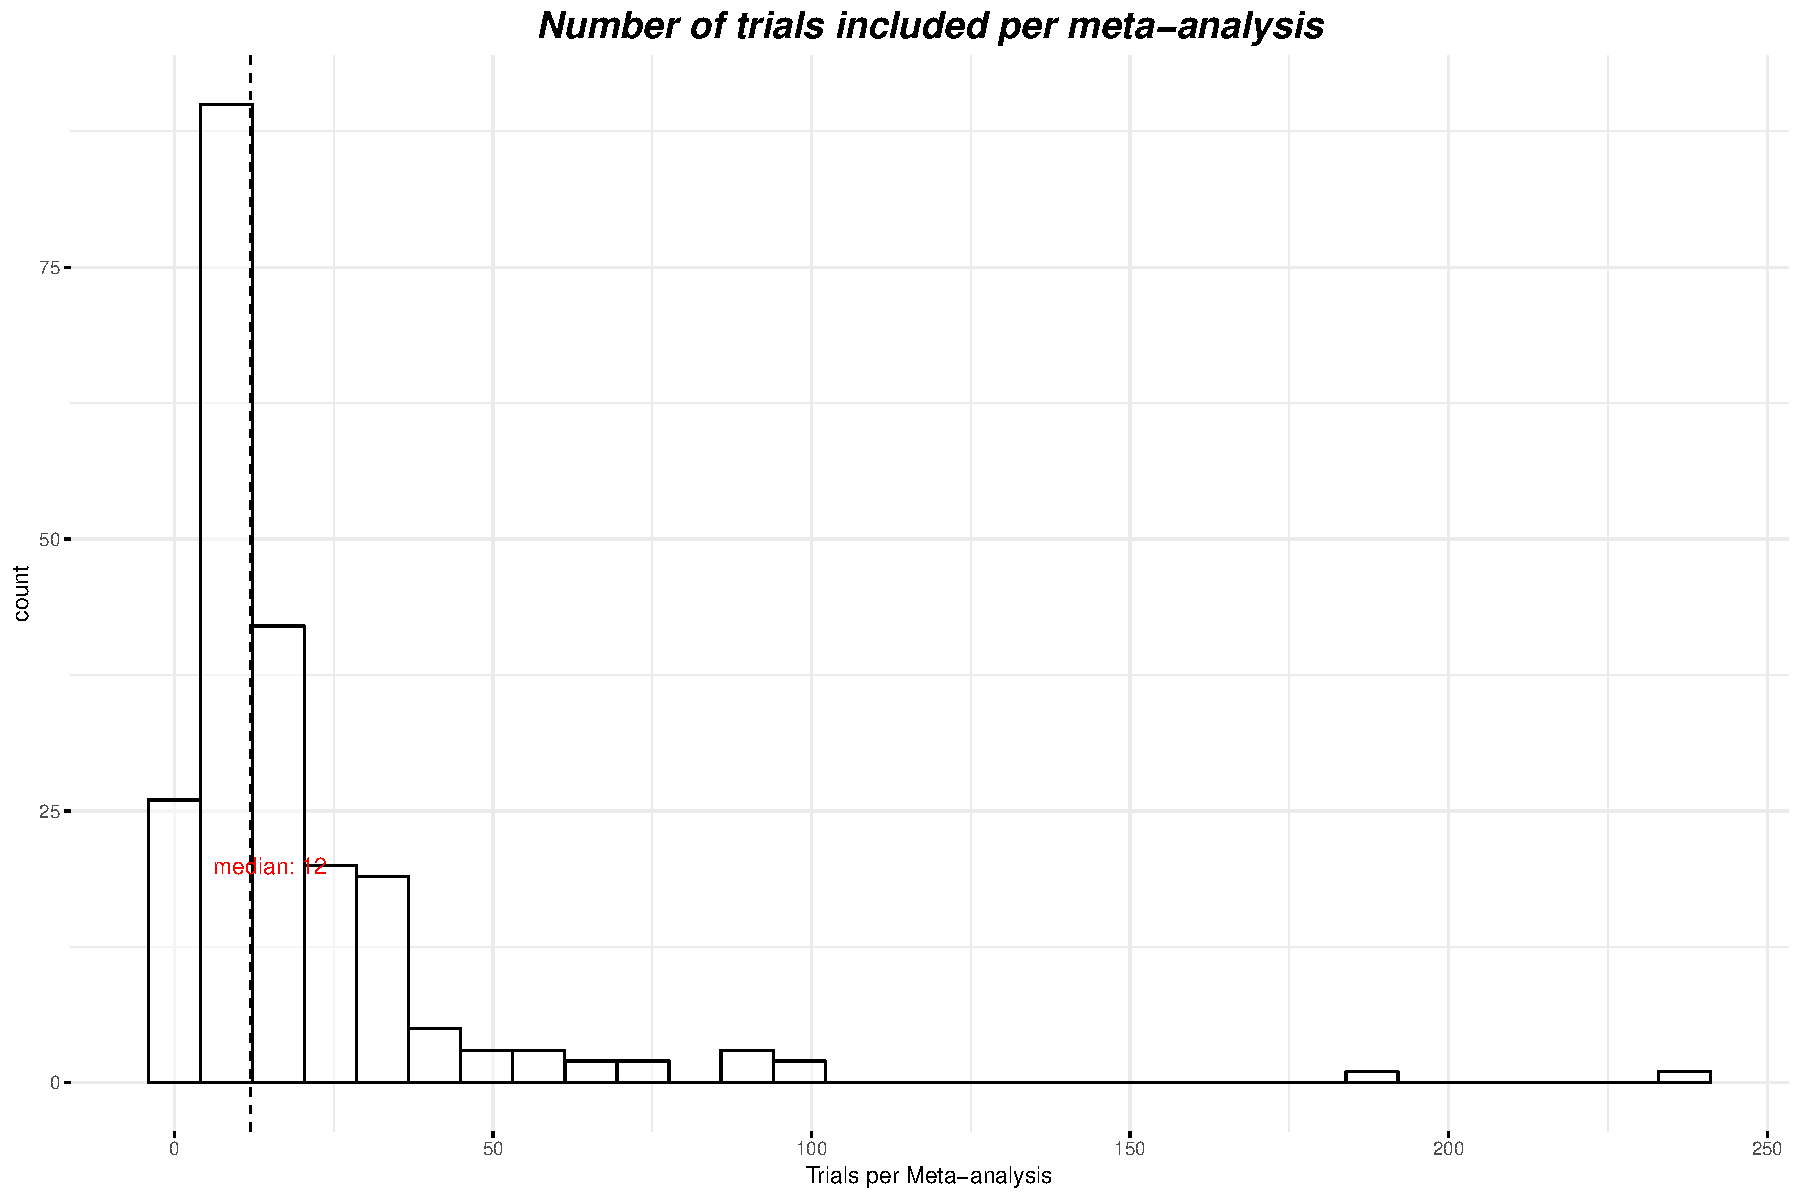
\includegraphics{Figs/unnamed-chunk-4-1.pdf}
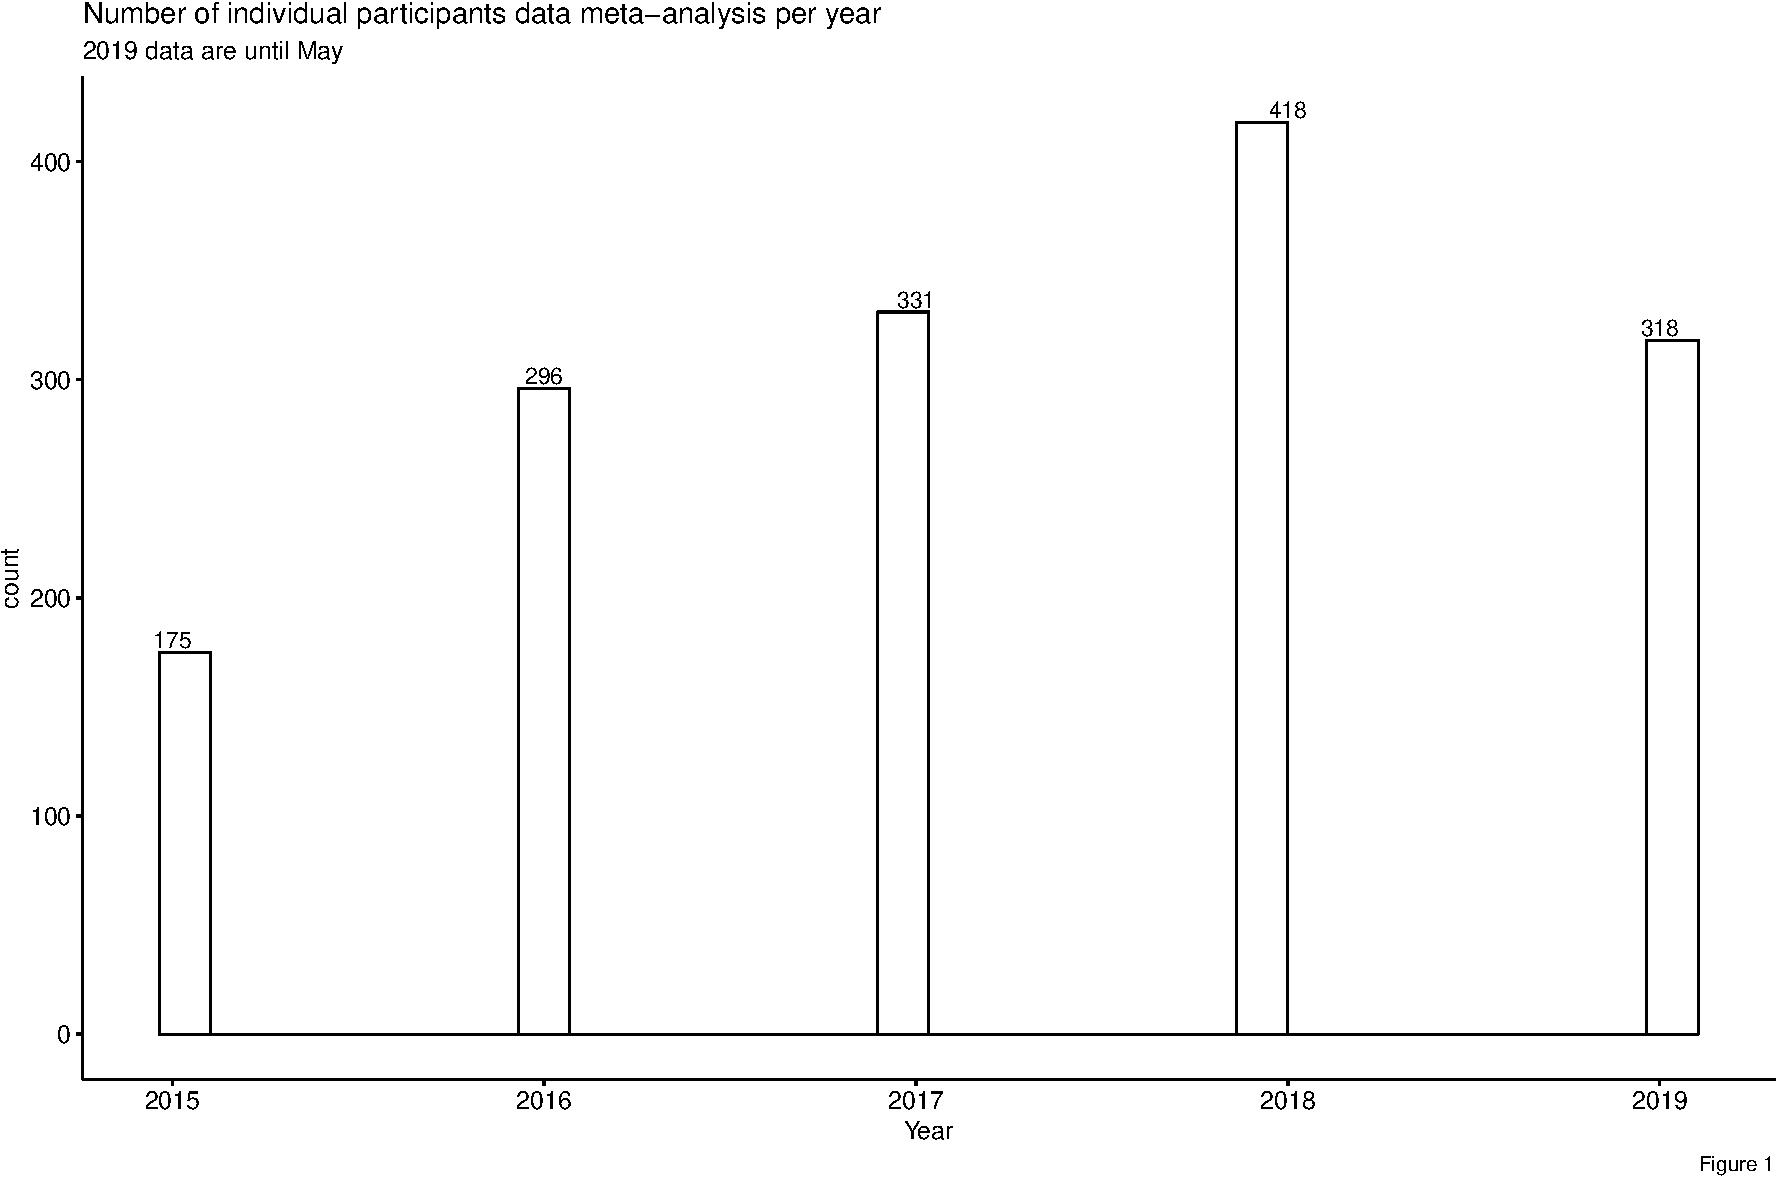
\includegraphics{Figs/unnamed-chunk-4-2.pdf}

\newpage

\hypertarget{references}{%
\section*{References}\label{references}}
\addcontentsline{toc}{section}{References}

\hypertarget{refs}{}
\leavevmode\hypertarget{ref-Stewart_1995}{}%
and, Lesley A. Stewart. 1995. ``Practical Methodology of Meta-Analyses
(Overviews) Using Updated Individual Patient Data.'' \emph{Statistics in
Medicine} 14 (19): 2057--79.
\url{https://doi.org/10.1002/sim.4780141902}.

\leavevmode\hypertarget{ref-CHALMERS_1993}{}%
CHALMERS, IAIN. 1993. ``The Cochrane Collaboration: Preparing,
Maintaining, and Disseminating Systematic Reviews of the Effects of
Health Care.'' \emph{Annals of the New York Academy of Sciences} 703 (1
Doing More Go): 156--65.
\url{https://doi.org/10.1111/j.1749-6632.1993.tb26345.x}.

\leavevmode\hypertarget{ref-Fisher_2011}{}%
Fisher, D. J., A. J. Copas, J. F. Tierney, and M. K.B. Parmar. 2011. ``A
Critical Review of Methods for the Assessment of Patient-Level
Interactions in Individual Participant Data Meta-Analysis of Randomized
Trials, and Guidance for Practitioners.'' \emph{Journal of Clinical
Epidemiology} 64 (9): 949--67.
\url{https://doi.org/10.1016/j.jclinepi.2010.11.016}.

\leavevmode\hypertarget{ref-Hua_2016}{}%
Hua, Hairui, Danielle L. Burke, Michael J. Crowther, Joie Ensor, Catrin
Tudur Smith, and Richard D. Riley. 2016. ``One-Stage Individual
Participant Data Meta-Analysis Models: Estimation of Treatment-Covariate
Interactions Must Avoid Ecological Bias by Separating Out Within-Trial
and Across-Trial Information.'' \emph{Statistics in Medicine} 36 (5):
772--89. \url{https://doi.org/10.1002/sim.7171}.

\leavevmode\hypertarget{ref-IntHout_2016}{}%
IntHout, Joanna, John P A Ioannidis, Maroeska M Rovers, and Jelle J
Goeman. 2016. ``Plea for Routinely Presenting Prediction Intervals in
Meta-Analysis.'' \emph{BMJ Open} 6 (7): e010247.
\url{https://doi.org/10.1136/bmjopen-2015-010247}.

\leavevmode\hypertarget{ref-Riley_2010}{}%
Riley, R. D., P. C. Lambert, and G. Abo-Zaid. 2010. ``Meta-Analysis of
Individual Participant Data: Rationale, Conduct, and Reporting.''
\emph{BMJ} 340 (feb05 1): c221--c221.
\url{https://doi.org/10.1136/bmj.c221}.

\leavevmode\hypertarget{ref-royston_interaction_2013}{}%
Royston, Patrick, and Willi Sauerbrei. 2013. ``Interaction of Treatment
with a Continuous Variable: Simulation Study of Significance Level for
Several Methods of Analysis.'' \emph{Statistics in Medicine} 32 (22):
3788--3803. \url{https://doi.org/10.1002/sim.5813}.

\leavevmode\hypertarget{ref-Sauerbrei_2011}{}%
Sauerbrei, Willi, and Patrick Royston. 2011. ``A New Strategy for
Meta-Analysis of Continuous Covariates in Observational Studies.''
\emph{Statistics in Medicine} 30 (28): 3341--60.
\url{https://doi.org/10.1002/sim.4333}.

\leavevmode\hypertarget{ref-Schuit_2018}{}%
Schuit, Ewoud, Alvin H Li, and John P A Ioannidis. 2018. ``How Often Can
Meta-Analyses of Individual-Level Data Individualize Treatment? A
Meta-Epidemiologic Study.'' \emph{International Journal of Epidemiology}
48 (2): 596--608. \url{https://doi.org/10.1093/ije/dyy239}.

\leavevmode\hypertarget{ref-Simmonds_2005}{}%
Simmonds, Mark C, Julian P T Higginsa, Lesley A Stewartb, Jayne F
Tierneyb, Mike J Clarke, and Simon G Thompson. 2005. ``Meta-Analysis of
Individual Patient Data from Randomized Trials: A Review of Methods Used
in Practice.'' \emph{Clinical Trials: Journal of the Society for
Clinical Trials} 2 (3): 209--17.
\url{https://doi.org/10.1191/1740774505cn087oa}.

\leavevmode\hypertarget{ref-Simmonds_2015}{}%
Simmonds, Mark, Gavin Stewart, and Lesley Stewart. 2015. ``A Decade of
Individual Participant Data Meta-Analyses: A Review of Current
Practice.'' \emph{Contemporary Clinical Trials} 45 (November): 76--83.
\url{https://doi.org/10.1016/j.cct.2015.06.012}.

\leavevmode\hypertarget{ref-Simmonds_2007}{}%
Simmonds, M. C., and J. P. T. Higgins. 2007. ``Covariate Heterogeneity
in Meta-Analysis: Criteria for Deciding Between Meta-Regression and
Individual Patient Data.'' \emph{Statistics in Medicine} 26 (15):
2982--99. \url{https://doi.org/10.1002/sim.2768}.

\leavevmode\hypertarget{ref-Stewart_1993}{}%
Stewart, L. A, and M. K.B Parmar. 1993. ``Meta-Analysis of the
Literature or of Individual Patient Data: Is There a Difference?''
\emph{The Lancet} 341 (8842): 418--22.
\url{https://doi.org/10.1016/0140-6736(93)93004-k}.

\leavevmode\hypertarget{ref-Stewart_2015}{}%
Stewart, Lesley A., Mike Clarke, Maroeska Rovers, Richard D. Riley, Mark
Simmonds, Gavin Stewart, and Jayne F. Tierney. 2015. ``Preferred
Reporting Items for a Systematic Review and Meta-Analysis of Individual
Participant Data.'' \emph{JAMA} 313 (16): 1657.
\url{https://doi.org/10.1001/jama.2015.3656}.

\leavevmode\hypertarget{ref-Stewart_2002}{}%
Stewart, Lesley A., and Jayne F. Tierney. 2002. ``To IPD or Not to
IPD?'' \emph{Evaluation \& the Health Professions} 25 (1): 76--97.
\url{https://doi.org/10.1177/0163278702025001006}.

\leavevmode\hypertarget{ref-van_Walraven_2010}{}%
Walraven, Carl van. 2010. ``Individual Patient Meta-Analysisrewards and
Challenges.'' \emph{Journal of Clinical Epidemiology} 63 (3): 235--37.
\url{https://doi.org/10.1016/j.jclinepi.2009.04.001}.


\end{document}
